\section[Fonctionnement]{Exemple de fonctionnement}

\begin{frame}{ Affichage via DirectFB }
	\begin{block} { Différence d'affichage entre les waveformes }
		\parbox{0.3\linewidth}{
			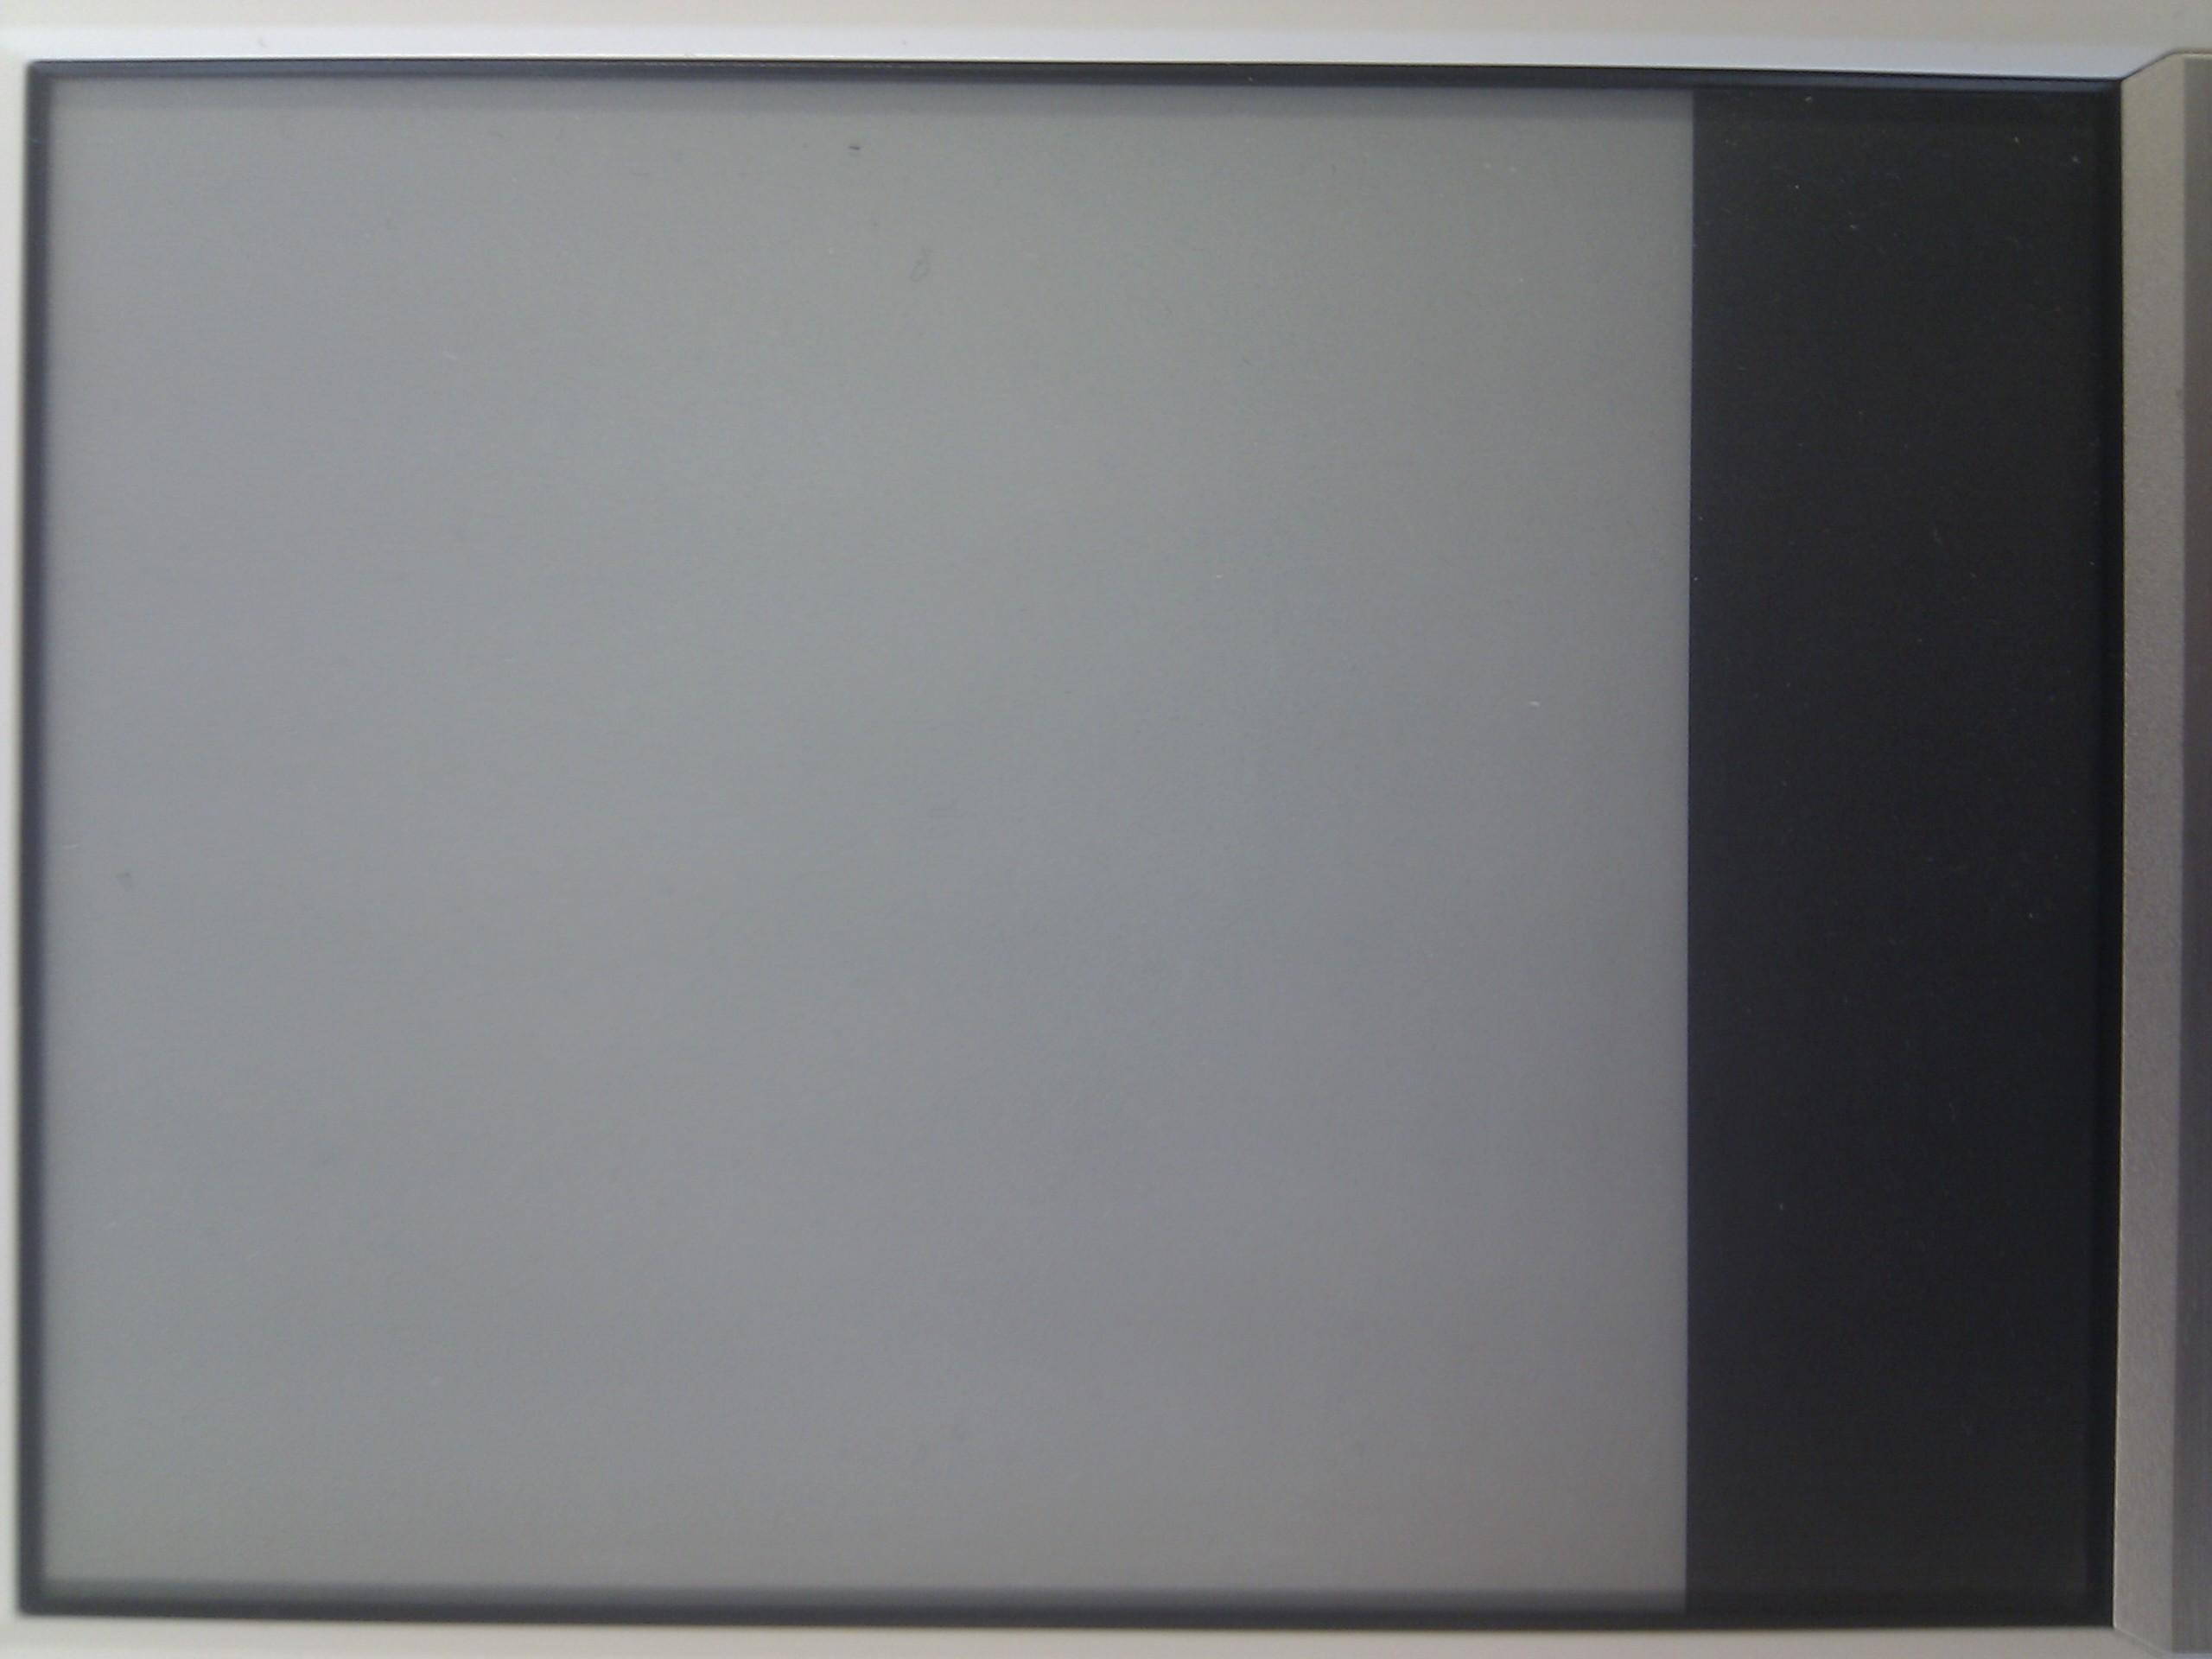
\includegraphics[angle=-90,origin=c,scale=0.04]{du_a2.jpg}
		}
		\parbox{0.6\linewidth}{
			\begin{itemize}
				\item DU ou A2
				\begin{itemize}
					\item seulement 2 niveaux de gris
					\item temps de rafraîchissement : 
					\begin{itemize}
						\item mesuré  : 126ms (A2) 280ms (DU)
						\item annoncé  : 300ms
					\end{itemize}		
				\end{itemize}
			\end{itemize}
		}
	\end{block}
\end{frame}

\begin{frame}{ Affichage via DirectFB }
	\begin{block} { Différence d'affichage entre les waveformes }
		\parbox{0.3\linewidth}{
			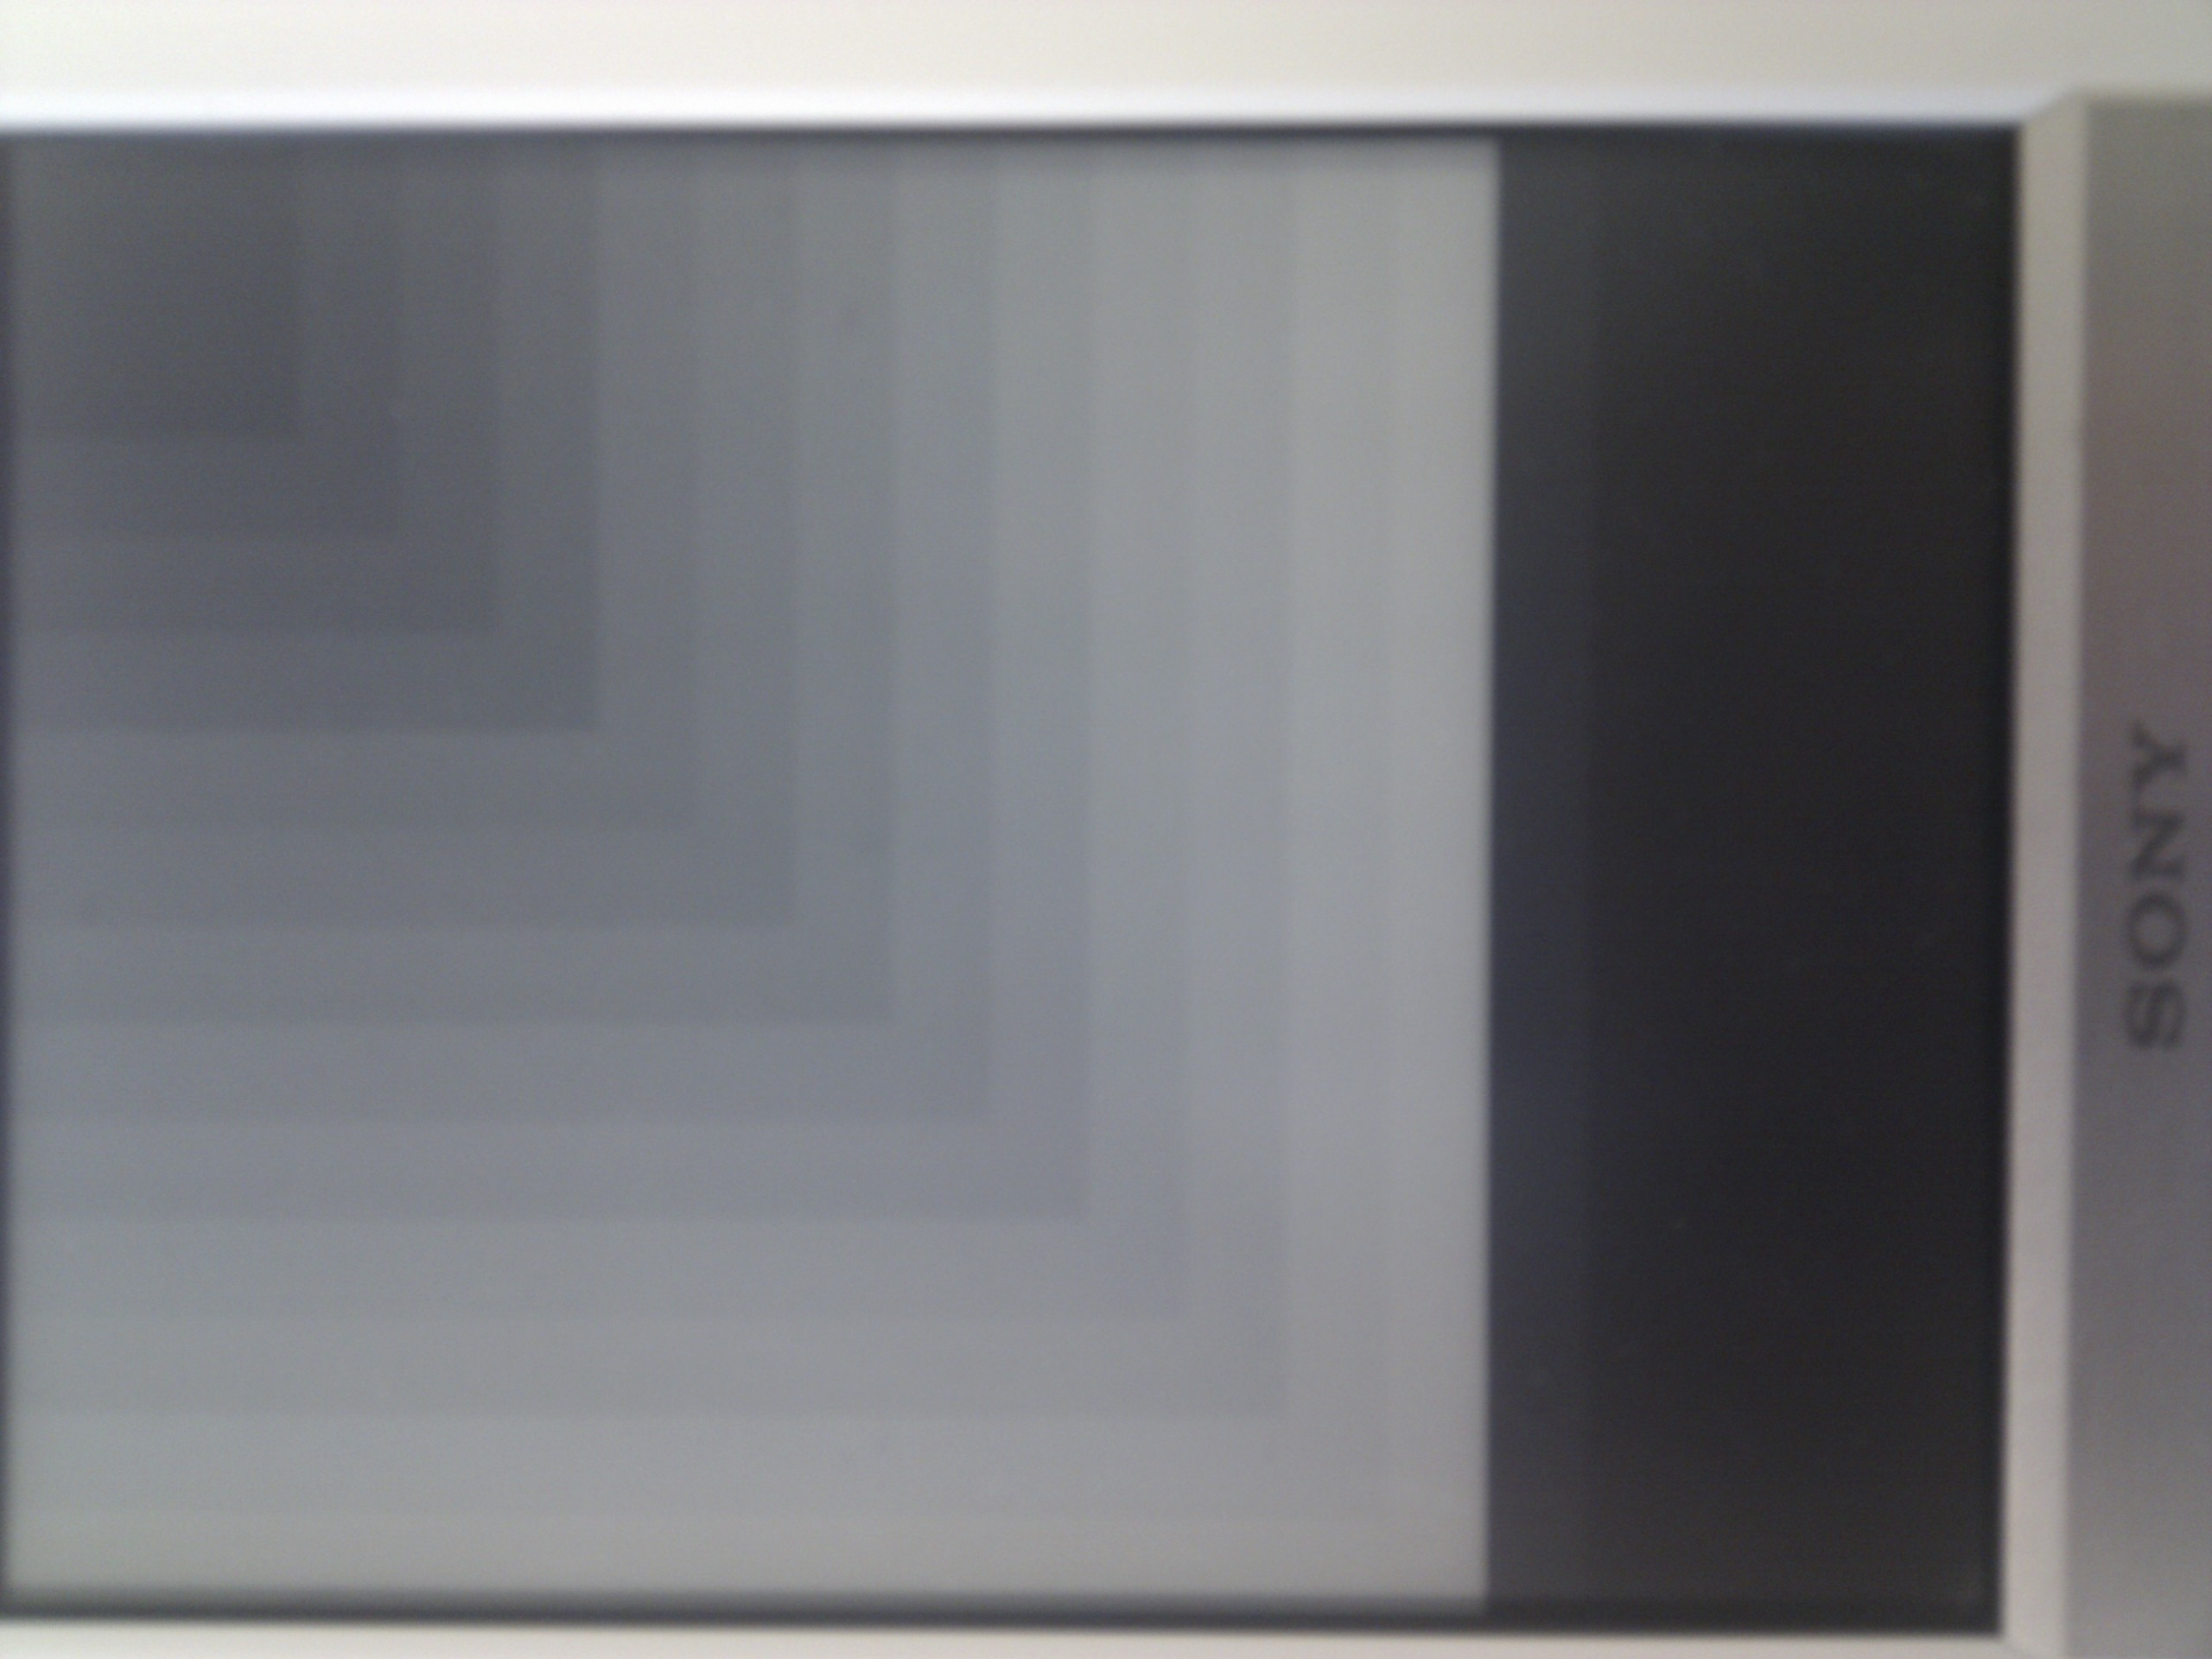
\includegraphics[angle=-90,origin=c,scale=0.04]{gc4_8.jpg}
		}
		\parbox{0.6\linewidth}{
			\begin{itemize}
				\item GC4
				\begin{itemize}
					\item 4 niveaux de gris
					\item temps de rafraîchissement : 
					\begin{itemize}
						\item mesuré  : 610ms
						\item annoncé  : 600ms
					\end{itemize}		
				\end{itemize}
			\end{itemize}
		}
	\end{block}
\end{frame}

\begin{frame}{ Affichage via DirectFB }
	\begin{block} { Différence d'affichage entre les waveformes }
		\parbox{0.3\linewidth}{
			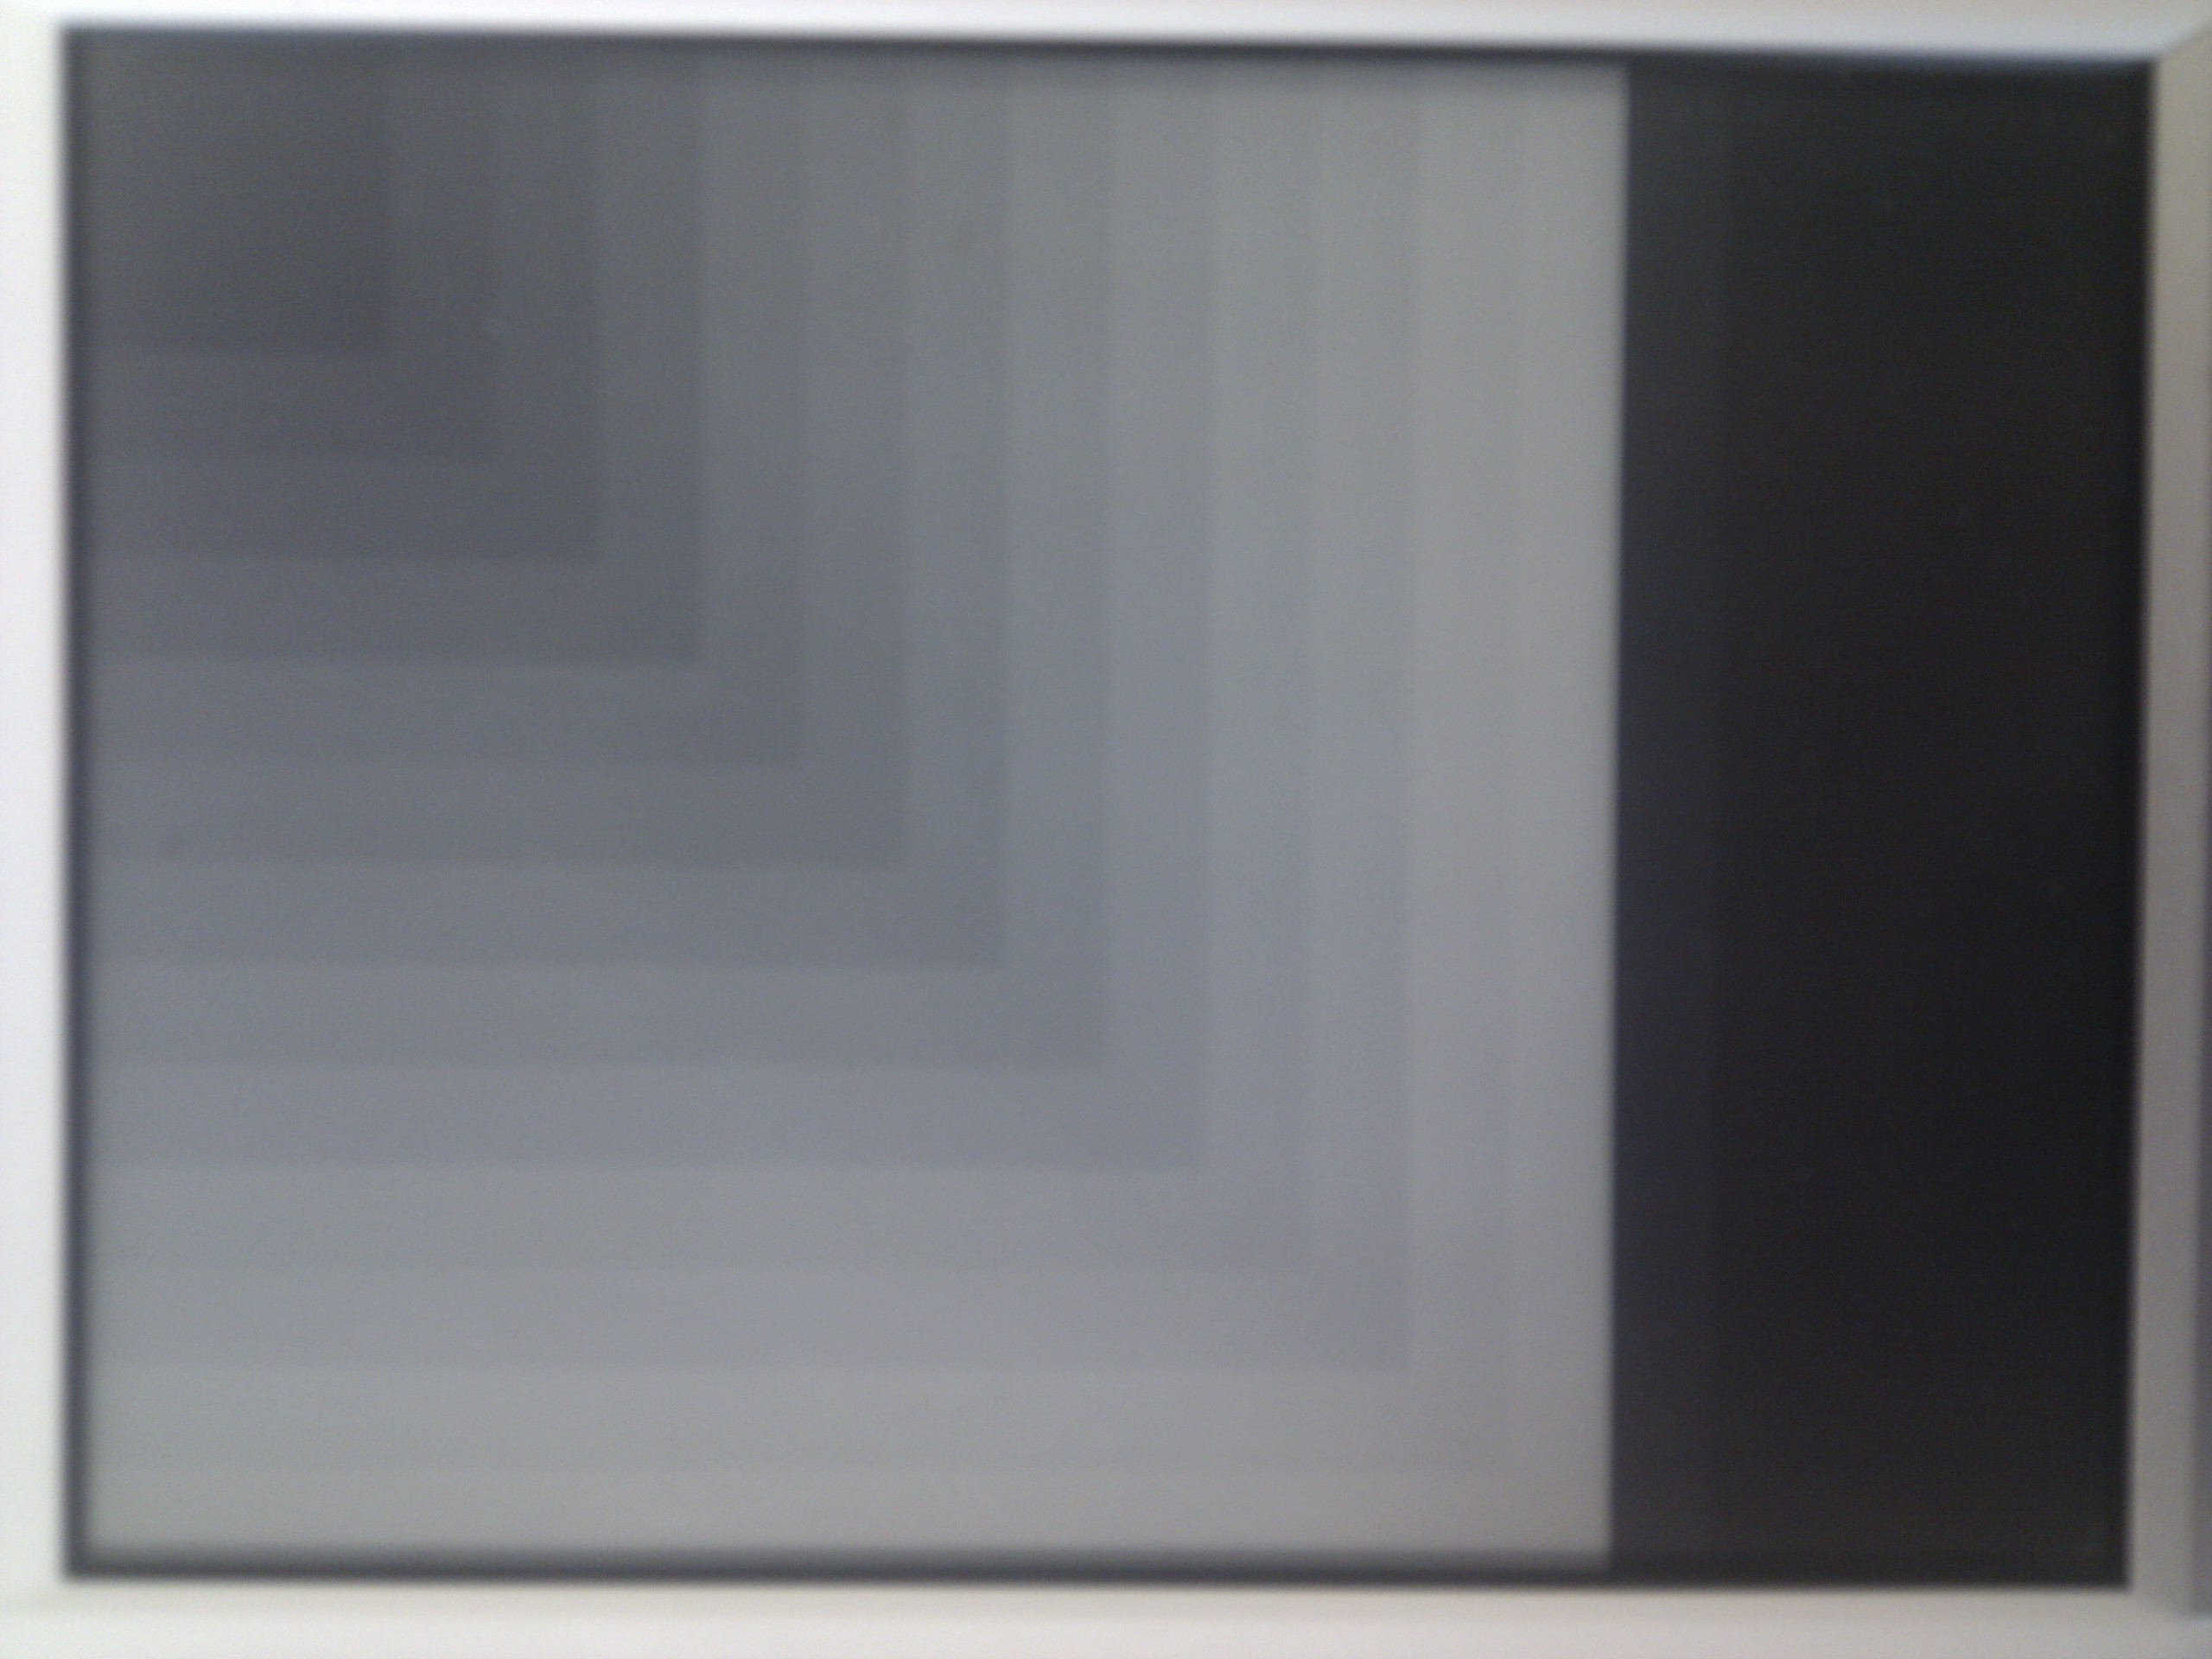
\includegraphics[angle=-90,origin=c,scale=0.04]{gc8_4.jpg}
		}
		\parbox{0.6\linewidth}{
			\begin{itemize}
				\item GC8 ou GC16
				\begin{itemize}
					\item 16 niveaux de gris
					\item temps de rafraîchissement : 
					\begin{itemize}
						\item mesuré  : 610ms
						\item annoncé  : 900ms
					\end{itemize}		
				\end{itemize}
			\end{itemize}
		}
	\end{block}
\end{frame}